

\tikzset{every picture/.style={line width=0.75pt}} %set default line width to 0.75pt        

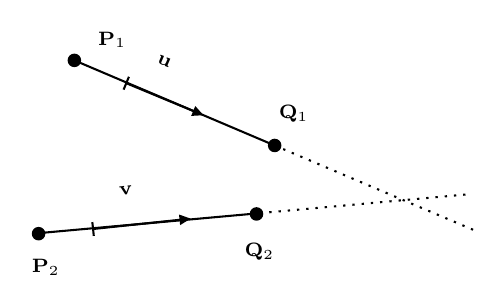
\begin{tikzpicture}[x=0.75pt,y=0.75pt,yscale=-1,xscale=1]
%uncomment if require: \path (0,300); %set diagram left start at 0, and has height of 300

%Straight Lines [id:da9380375306195725] 
\draw    (151,60.75) -- (178.91,72.61) -- (247.5,101.75) ;
%Straight Lines [id:da58454089790185] 
\draw  [dash pattern={on 0.84pt off 2.51pt}]  (247.5,101.75) -- (344,142.75) ;
%Straight Lines [id:da4212167048643327] 
\draw    (131,144.25) -- (236,134.75) ;
%Straight Lines [id:da027822666102904292] 
\draw  [dash pattern={on 0.84pt off 2.51pt}]  (236,134.75) -- (341,125.25) ;
%Shape: Circle [id:dp14206980425238902] 
\draw  [fill={rgb, 255:red, 0; green, 0; blue, 0 }  ,fill opacity=1 ] (244.75,101.75) .. controls (244.75,100.23) and (245.98,99) .. (247.5,99) .. controls (249.02,99) and (250.25,100.23) .. (250.25,101.75) .. controls (250.25,103.27) and (249.02,104.5) .. (247.5,104.5) .. controls (245.98,104.5) and (244.75,103.27) .. (244.75,101.75) -- cycle ;
%Shape: Circle [id:dp2202026658580638] 
\draw  [fill={rgb, 255:red, 0; green, 0; blue, 0 }  ,fill opacity=1 ] (148.25,60.75) .. controls (148.25,59.23) and (149.48,58) .. (151,58) .. controls (152.52,58) and (153.75,59.23) .. (153.75,60.75) .. controls (153.75,62.27) and (152.52,63.5) .. (151,63.5) .. controls (149.48,63.5) and (148.25,62.27) .. (148.25,60.75) -- cycle ;
%Shape: Circle [id:dp016326297271163193] 
\draw  [fill={rgb, 255:red, 0; green, 0; blue, 0 }  ,fill opacity=1 ] (236,134.75) .. controls (236,133.23) and (237.23,132) .. (238.75,132) .. controls (240.27,132) and (241.5,133.23) .. (241.5,134.75) .. controls (241.5,136.27) and (240.27,137.5) .. (238.75,137.5) .. controls (237.23,137.5) and (236,136.27) .. (236,134.75) -- cycle ;
%Shape: Circle [id:dp6460481311401347] 
\draw  [fill={rgb, 255:red, 0; green, 0; blue, 0 }  ,fill opacity=1 ] (131,144.25) .. controls (131,142.73) and (132.23,141.5) .. (133.75,141.5) .. controls (135.27,141.5) and (136.5,142.73) .. (136.5,144.25) .. controls (136.5,145.77) and (135.27,147) .. (133.75,147) .. controls (132.23,147) and (131,145.77) .. (131,144.25) -- cycle ;
%Straight Lines [id:da9398932028593516] 
\draw    (176,71.75) -- (210.43,86.03) ;
\draw [shift={(213.21,87.18)}, rotate = 202.52] [fill={rgb, 255:red, 0; green, 0; blue, 0 }  ][line width=0.08]  [draw opacity=0] (5.36,-2.57) -- (0,0) -- (5.36,2.57) -- cycle    ;
\draw [shift={(176,71.75)}, rotate = 202.52] [color={rgb, 255:red, 0; green, 0; blue, 0 }  ][line width=0.75]    (0,3.35) -- (0,-3.35)   ;
%Straight Lines [id:da192790896951491] 
\draw    (160,142) -- (204.02,137.32) ;
\draw [shift={(207,137)}, rotate = 173.93] [fill={rgb, 255:red, 0; green, 0; blue, 0 }  ][line width=0.08]  [draw opacity=0] (5.36,-2.57) -- (0,0) -- (5.36,2.57) -- cycle    ;
\draw [shift={(160,142)}, rotate = 173.93] [color={rgb, 255:red, 0; green, 0; blue, 0 }  ][line width=0.75]    (0,3.35) -- (0,-3.35)   ;

% Text Node
\draw (161,45.5) node [anchor=north west][inner sep=0.75pt]  [font=\scriptsize] [align=left] {$\mathbf{P}_1$};
% Text Node
\draw (248,81) node [anchor=north west][inner sep=0.75pt]  [font=\scriptsize] [align=left] {$\mathbf{Q}_1$};
% Text Node
\draw (129,155) node [anchor=north west][inner sep=0.75pt]  [font=\scriptsize] [align=left] {$\mathbf{P}_2$};
% Text Node
\draw (231.5,147.5) node [anchor=north west][inner sep=0.75pt]  [font=\scriptsize] [align=left] {$\mathbf{Q}_2$};
% Text Node
\draw (170.7,120.28) node [anchor=north west][inner sep=0.75pt]  [font=\scriptsize,rotate=-353.99] [align=left] {$\displaystyle \mathbf{v}$};
% Text Node
\draw (191.22,55.89) node [anchor=north west][inner sep=0.75pt]  [font=\scriptsize,rotate=-23.19] [align=left] {$\displaystyle \mathbf{u}$};


\end{tikzpicture}
